\documentclass{article}
\usepackage{graphicx} % Required for inserting images
\usepackage{float}
\usepackage[T1]{fontenc}
\usepackage{amsmath}
\usepackage[margin=1in]{geometry}
\usepackage{booktabs}
\usepackage{tabularx}
\usepackage[hidelinks]{hyperref}

\title{A 10-share hedge band on the SPY gamma book}
\author{Experiment report \textperiodcentered{} L/S Gamma Desk, QUANTT}
\date{2026-10-16}

\begin{document}

\maketitle

\textbf{Question:} Does re-hedging only when the delta drift reaches 10 shares (a hedge band) give higher net P\&L than re-hedging every share, because it cuts \$1-minimum hedge orders, without a worse tail?

\textbf{Method:} Pre-registered backtest (the hypothesis card was committed before any run). The live paper rules (\texttt{configs/\allowbreak{}paper.\allowbreak{}toml}) are replayed on R2 replay snapshots v1 (config\_hash b040760187f0) over the development window 2014-06-02 to 2024-12-31. The hold-out (2025-01-01 to 2026-07-10) was not used. The only change is \texttt{[hedge] min\_\allowbreak{}shares}: at each hedge time (10:15 ET, once a day, as live) the engine skips the rebalance when |target \ensuremath{-} held| < \texttt{min\_\allowbreak{}shares}, and otherwise trades the full difference back to the delta target. This is the same rule as the live \texttt{portfolio.\allowbreak{}rebalance}. Variants: \texttt{band5}, \texttt{band10} (primary, the only one the pass bar uses) and \texttt{band20}, with \texttt{min\_\allowbreak{}shares} of 5, 10 and 20. The baseline is trial 1 of the \texttt{baseline} experiment (\texttt{min\_\allowbreak{}shares = 1}). Each variant ran once at 1x and 2x spreads and is compared with the baseline at the same spread multiple. Costs are \$0.65 per contract and \$0.005 per share, with a \$1 minimum per order. One contract, so almost every hedge order pays the \$1 minimum.

\begin{quote}This report was written by Claude at the PM's request.\end{quote}

\section{Result vs the pass bar}

Both bars had to hold at both 1x and 2x. P\&L is net USD for one contract. ES is the mean of the worst 5\% of daily net P\&L.

\begin{center}\small
\begin{tabularx}{\linewidth}{>{\raggedright\arraybackslash}X >{\raggedright\arraybackslash}X >{\raggedright\arraybackslash}X l}
\toprule
\textbf{Bar} & \textbf{1x: band10 vs baseline} & \textbf{2x: band10 vs baseline} & \textbf{Result} \\
\midrule
1. Net P\&L > baseline, full window & \ensuremath{-}1,096.9 vs \ensuremath{-}2,059.5 & \ensuremath{-}3,258.5 vs \ensuremath{-}4,122.3 & pass \\
1. Net P\&L > baseline, 2014-06 to 2019-12 & \ensuremath{-}779.7 vs \ensuremath{-}986.2 & \ensuremath{-}1,408.5 vs \ensuremath{-}1,511.3 & pass \\
1. Net P\&L > baseline, 2020-01 to 2024-12 & \ensuremath{-}317.2 vs \ensuremath{-}1,073.3 & \ensuremath{-}1,850.0 vs \ensuremath{-}2,610.9 & pass \\
2. abs(ES 5\%) \ensuremath{\leq} 1.10 \ensuremath{\times} baseline, full window & 98.1 vs 96.5 (1.02\ensuremath{\times}) & 106.8 vs 104.5 (1.02\ensuremath{\times}) & pass \\
\bottomrule
\end{tabularx}
\end{center}

\textbf{Verdict: passed} at both spread multiples. The book still loses money: band10 cuts the 1x loss by \$963 (47\%) and the 2x loss by \$864 (21\%), but it does not make the strategy profitable.

Other numbers, not part of the bar:

\begin{center}\small
\begin{tabularx}{\linewidth}{>{\raggedright\arraybackslash}X l l l l l}
\toprule
\textbf{Full window} & \textbf{baseline 1x} & \textbf{band5 1x} & \textbf{band10 1x} & \textbf{band20 1x} & \textbf{band10 2x} \\
\midrule
Net P\&L & \ensuremath{-}2,059.5 & \ensuremath{-}1,665.5 & \ensuremath{-}1,096.9 & \ensuremath{-}2,224.1 & \ensuremath{-}3,258.5 \\
Sharpe & \ensuremath{-}0.36 & \ensuremath{-}0.29 & \ensuremath{-}0.19 & \ensuremath{-}0.32 & \ensuremath{-}0.53 \\
Max drawdown & 3,027 & 3,000 & 2,505 & 3,348 & 3,412 \\
ES 5\% (daily) & \ensuremath{-}96.5 & \ensuremath{-}96.0 & \ensuremath{-}98.1 & \ensuremath{-}116.9 & \ensuremath{-}106.8 \\
Hedge orders (= hedge fees, USD) & 914 & 666 & 469 & 303 & 469 \\
Median shares per order & 9 & 13 & 21 & 47 & 21 \\
Round trips & 131 & 131 & 131 & 132 & 131 \\
\bottomrule
\end{tabularx}
\end{center}

The sensitivity variants do not change the verdict, but they matter for reading it. \texttt{band5} gains less (\$394 at 1x). \texttt{band20} is worse than the baseline at both multiples and its ES is about 1.2\ensuremath{\times} the baseline's, so it would have failed both bars.

\section{Charts}

\begin{figure}[H]\centering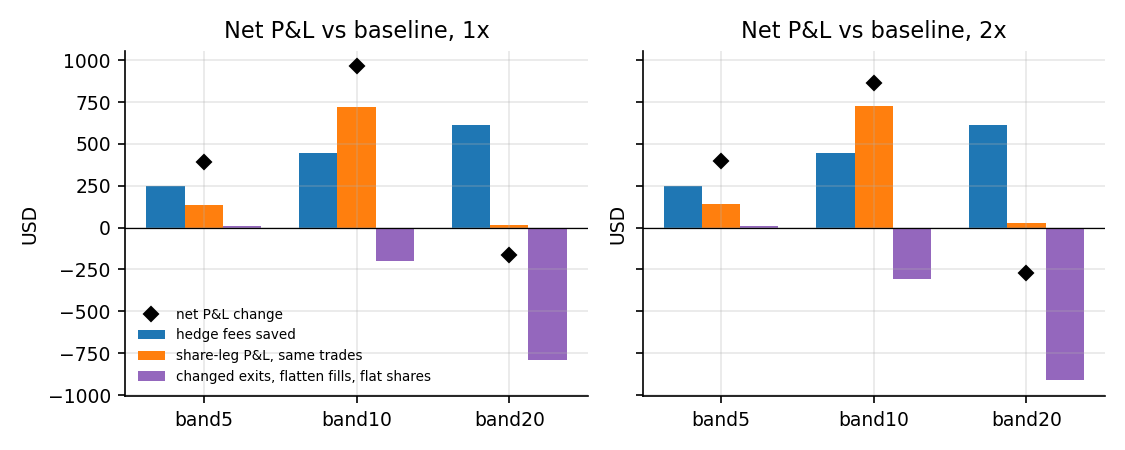
\includegraphics[width=0.92\linewidth]{figures/pnl_bridge.png}\caption{Net P\&L change vs the baseline, split into hedge fees saved, share-leg P\&L on round trips that are the same in both runs, and the rest (round trips with a different exit, flattening fills after a close, shares left on while flat).}\end{figure}

This chart answers whether the band changes hedging P\&L or only fees. At band10, \$445 of the \$963 gain (1x) is fees saved. Another \$717 comes from the share leg of the 130 round trips that are identical in both runs, so the hedging P\&L itself improved. One short trade that hit a stop under band10 gives back \$200 (1x) and \$307 (2x). For band20 the fee saving (\$611) is wiped out by two stops and a changed trade.

\begin{figure}[H]\centering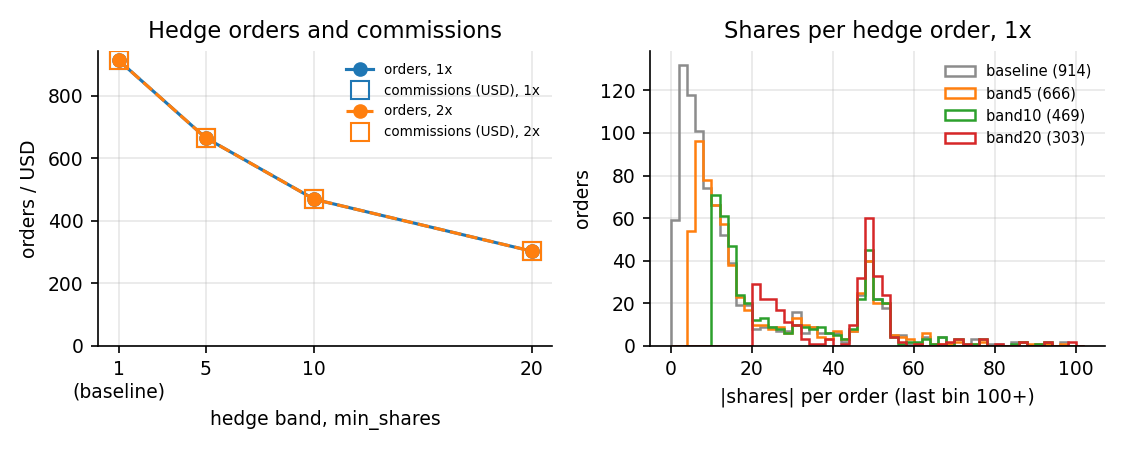
\includegraphics[width=0.92\linewidth]{figures/hedging.png}\caption{Left: hedge orders and hedge commissions vs the band at 1x and 2x (all four series coincide: each order pays the \$1 minimum, and the hedge orders are identical at 1x and 2x). Right: shares per hedge order for each band, 1x (2x is the same).}\end{figure}

Orders, and with them commissions, fall from 914 to 666, 469 and 303 as the band widens. An order of under 200 shares always pays the \$1 minimum. Each step of band removes fewer orders (248, then 197, then 166). The baseline is dominated by orders of 1 to 10 shares (median 9), and a band removes exactly these. The hump near 50 shares is mostly the first hedge after opening a near-the-money option (79\% of baseline orders of 40 to 60 shares), and no band removes it.

\begin{figure}[H]\centering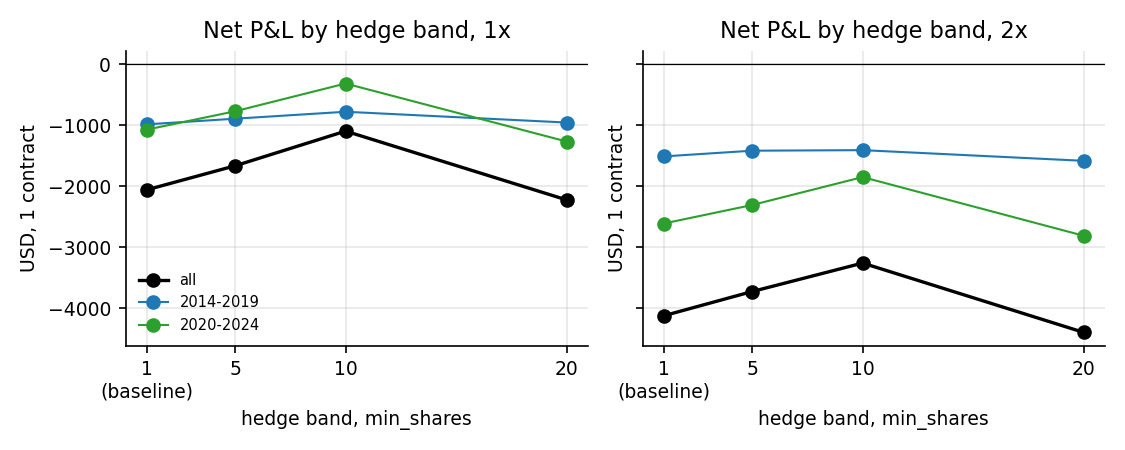
\includegraphics[width=0.92\linewidth]{figures/pnl_vs_band.png}\caption{Net P\&L vs the band, full window and both halves, 1x and 2x.}\end{figure}

Net P\&L peaks at band10 in both halves and at both multiples, and band20 falls back below the baseline. The first-half gain at 2x is small (\$103), smaller than the \$147 of fees saved in that half, because the 2015 stop lands there.

\begin{figure}[H]\centering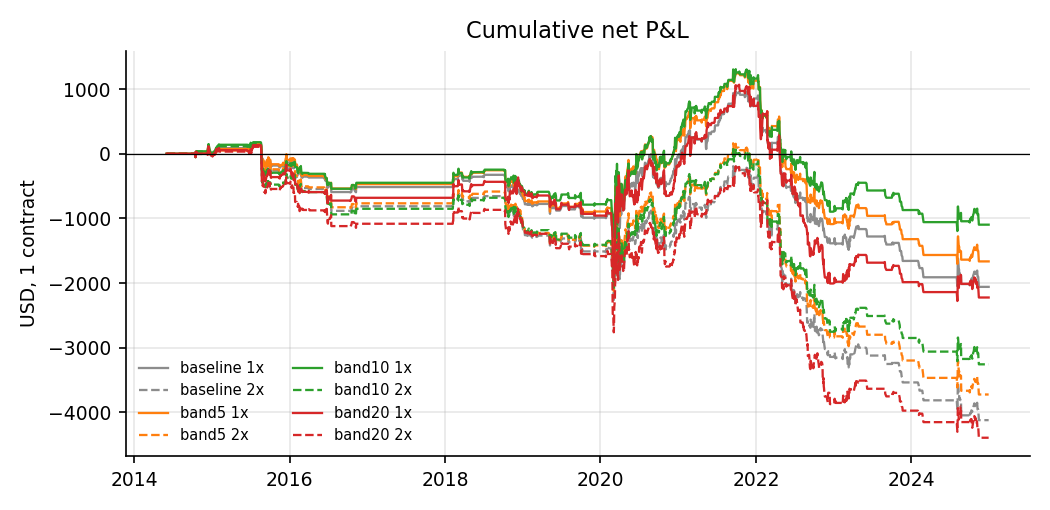
\includegraphics[width=0.92\linewidth]{figures/cum_pnl.png}\caption{Cumulative net P\&L, baseline and the three bands, 1x (solid) and 2x (dashed).}\end{figure}

The curves move together, since the trades are almost the same. Most of band10's lead builds from 2022 to 2024 (\$655 of the \$963 at 1x). All curves end below zero.

\begin{figure}[H]\centering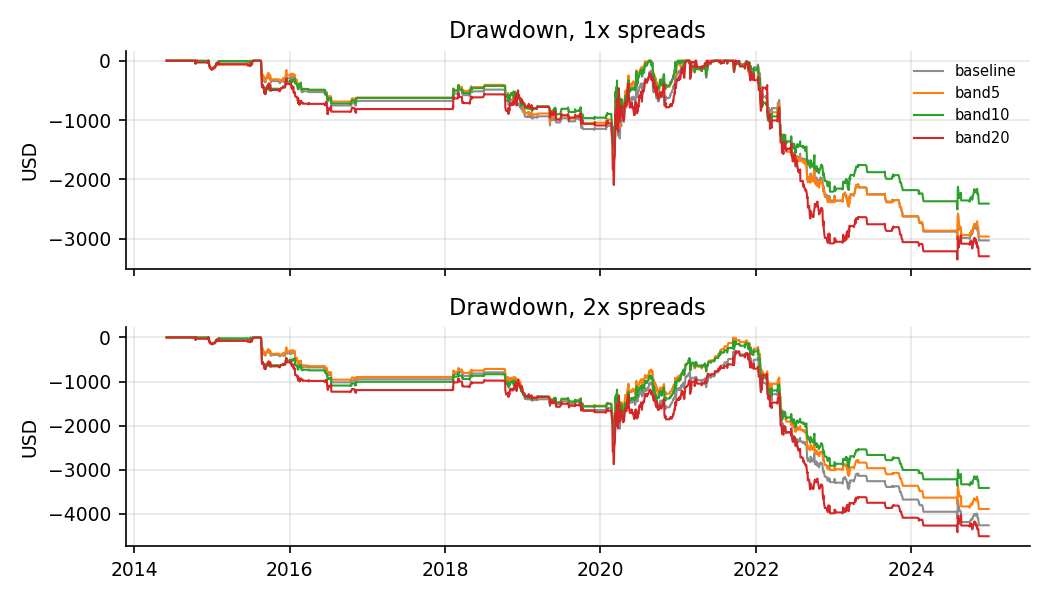
\includegraphics[width=0.92\linewidth]{figures/drawdown.png}\caption{Drawdown from the running peak, 1x and 2x.}\end{figure}

band10 has the shallowest drawdown at both multiples (2,505 vs 3,027 at 1x). band20 has the deepest (trough 2024-08-05); 2022 is its worst year.

\begin{figure}[H]\centering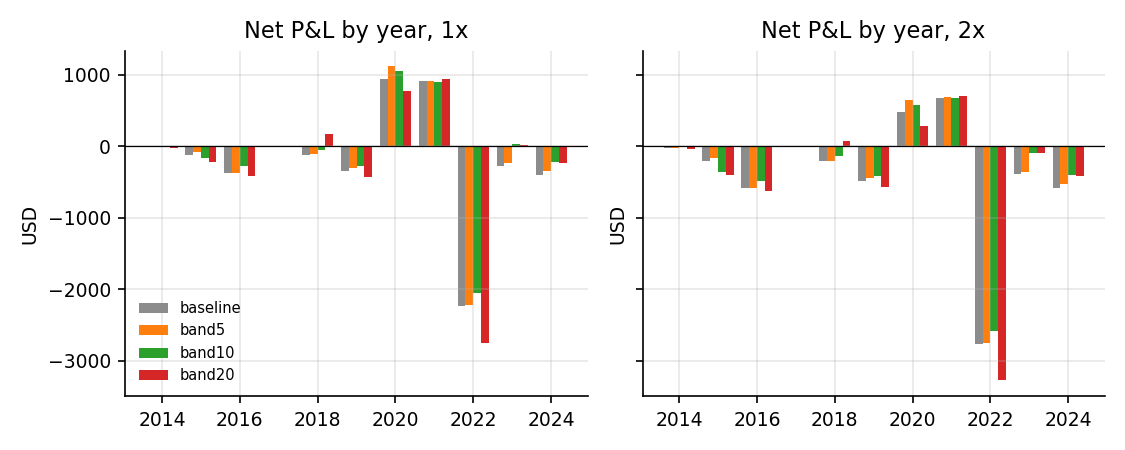
\includegraphics[width=0.92\linewidth]{figures/yearly.png}\caption{Net P\&L by year, 1x and 2x.}\end{figure}

No single year explains the band10 gain: at 1x it is ahead of the baseline in 8 of the 10 years with trades, and behind only in 2015 (the stop) and 2021, by less than \$50 each. 2022 is the worst year for every variant, and band20 loses the most there.

\begin{figure}[H]\centering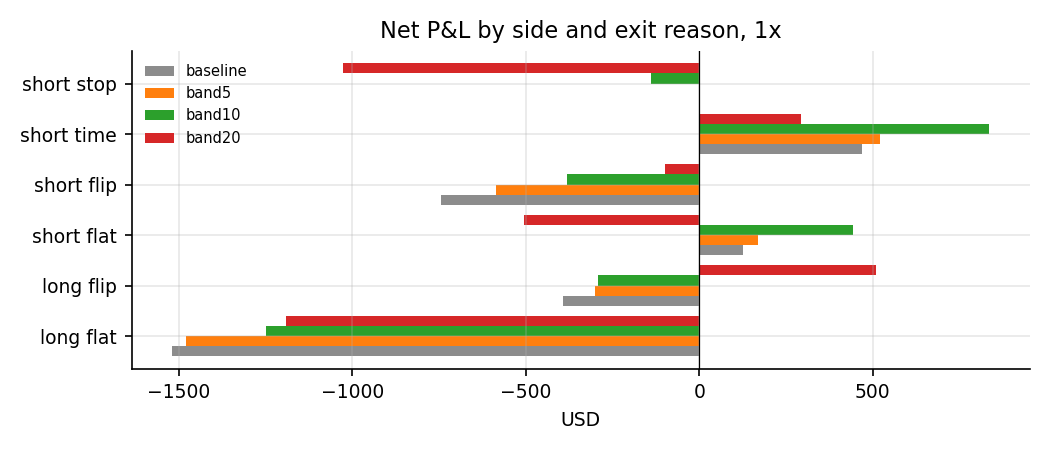
\includegraphics[width=0.92\linewidth]{figures/by_reason.png}\caption{Net P\&L by side and exit reason, 1x.}\end{figure}

The baseline never hit a stop in ten years. With a band, the combined option-plus-hedge P\&L of a short drifts further before it is re-hedged, and band10 hit one stop (2015) and band20 two. Under band10, longs and shorts both improve.

\begin{figure}[H]\centering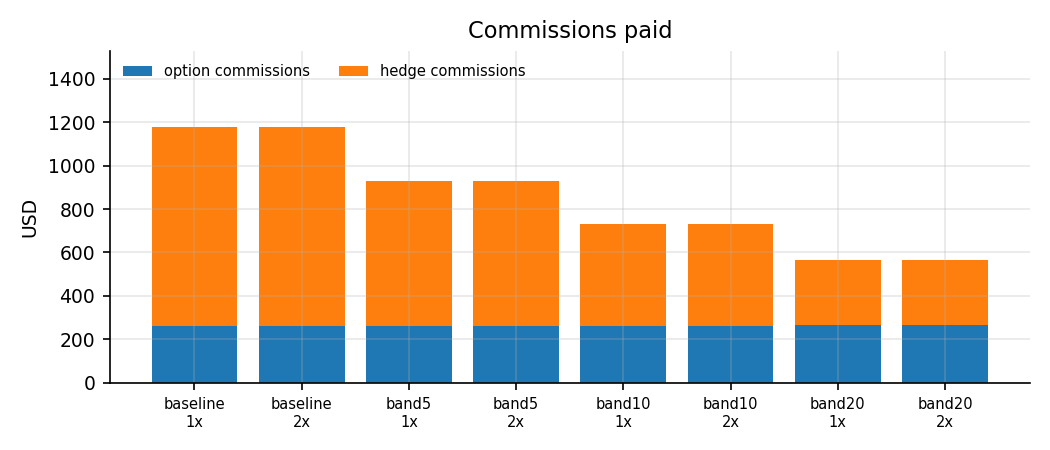
\includegraphics[width=0.92\linewidth]{figures/fees.png}\caption{Commissions paid, option and hedge, 1x and 2x.}\end{figure}

Option commissions stay at \$262 (band20: \$264, one extra round trip). Hedge commissions fall from \$914 to \$469 at band10, which brings total fees from \$1,176 to \$731.

\section{Analysis}

The fee saving is the mechanical part of the result and the part to trust. With one contract, every hedge order costs \$1 whatever its size, so skipping orders of under 10 shares saves \$445 over ten years. That alone would have cleared bar 1 in both halves, since the saving is positive in every period.

The larger part of the gain, \$717 at 1x, is a better share-leg P\&L on the 130 round trips that are otherwise identical. It is positive for longs and shorts and in both halves. But it does not grow steadily with the band: it is \$138 at band5, \$717 at band10 and only \$13 at band20, where longs gain \$1,117 and shorts lose \$1,104. In theory a band does not change the expected hedging P\&L, only its variance, so this part is most likely path noise that happens to favour band10 on this window. Expect it to be smaller, or of either sign, on the hold-out.

The cost of a band is a looser hedge. The engine's stop compares the combined option-plus-hedge P\&L with the credit, so a short that drifts while unhedged can reach the stop sooner. That happened once at band10 (2015) and twice at band20 (2015 and 2020). Most of the ``rest'' bar comes from those stops, including the flattening hedge after the band10 stop, which filled about \$4 per share away from the 15-minute-stale decision snapshot during a fast market (the typical gap is about \$0.56). Leftover shares while flat are not a factor at band10: every close left at least 10 shares to unwind, so the book was never flat with shares on. Only band20 held some, on 6 flat days (0.05 shares on average over all flat time), and they made \$180.

\section{Verdict}

\textbf{Passed.} band10 beats the baseline on net P\&L over the full window and in both halves, at both 1x and 2x, and its daily 5\% ES is 1.02\ensuremath{\times} the baseline's, well inside the 1.10\ensuremath{\times} limit. \$445 of the \$963 gain (1x) is the mechanical fee saving. The rest is a better hedging P\&L (\$717, partly given back by one stop), which the band5 and band20 runs suggest is not reliable. This is in-sample evidence only (see Caveats). The next step is the one hold-out run that the card requires.

\section{Caveats}

\begin{itemize}

\item \textbf{In-sample idea.} The idea came from the baseline's hedge-fee total on this same window, so the pass is in-sample evidence. Promotion needs one hold-out run with the same bar.

\item \textbf{Picking the peak.} Three bands were run and the primary sits at the best of them. The pass bar used band10 only and was fixed in advance, but P\&L peaking at the pre-chosen point is partly luck.

\item \textbf{One contract.} The \$1 minimum is large relative to a 1-contract book. At larger size, orders exceed 200 shares, the per-share fee takes over, and the saving from a band shrinks.

\item \textbf{Spread model.} Option and share spreads come from a model fitted on about two weeks of calm 2026 live quotes. 2x spreads are the stress check.

\item \textbf{Missing snapshots.} Month-end R2 days are missing (3.3\% of scheduled times skipped), the same for every variant.

\item \textbf{Hedge timing.} Hedges are checked once a day at 10:15 ET, as live. A band behaves differently with intraday hedging. Fills are on trades after a 15-minute-stale decision snapshot, and in fast markets a fill can be several dollars per share away from the decision price.

\item \textbf{Stops depend on the hedge.} Because the stop uses option-plus-hedge P\&L, a band changes when stops fire. In this window that changed 1 round trip at band10 and 2 at band20, so a few events drive the ``rest'' component.

\end{itemize}

\section{Trials}

8 trials in total: 6 for this experiment (\texttt{band5}, \texttt{band10} and \texttt{band20}, each at 1x and 2x, one run each) plus the baseline's 2. The baseline regression check that reproduced trial 1 was not registered. The first run's report step failed on a registry read while the three parallel experiments were writing to it, after all six trials had been registered. The report was then rebuilt from those runs with \texttt{-\allowbreak{}-\allowbreak{}report-\allowbreak{}only}, which creates no trials. After the run, a P\&L split (the bridge chart) was added to the report code. It reads the registered runs only, and the pass bar was not changed.

\end{document}
